\documentclass[12pt]{article}

\usepackage{enumerate}
\usepackage{rotating}
\usepackage{multicol}
\usepackage{multirow}
\usepackage{graphicx}
\usepackage{fullpage}
\usepackage{subfigure}
\usepackage{setspace}
\usepackage{listings}
\usepackage{lastpage}

\graphicspath{{./images/}}

% for references
\usepackage[pagebackref=false,colorlinks,linkcolor=blue,citecolor=magenta]{hyperref}
\usepackage[nottoc]{tocbibind}
\usepackage{fancyhdr}
\setlength{\headsep}{25pt}

\pagestyle{fancy}
\fancyhf{}
\lhead{\lr{Digital Image Processing}}
\rhead{تمرین دوم}
\cfoot{صفحه \thepage\ از \pageref{LastPage}}
\lfoot{نیمسال مهر 00-99}
\rfoot{حمیدرضا ابوئی مهریزی}


% xepersian
\usepackage[extrafootnotefeatures]{xepersian}
\settextfont[Scale=1.4]{B Nazanin}
\setlatintextfont{Times New Roman}

\renewcommand{\labelitemi}{$\bullet$}

\begin{document}
	\doublespacing
	\begin{titlepage}
		\paragraph*{}
		\centering
			
			
			{\small به نام او}\\
			\vspace{1cm}
			\includegraphics[width=0.12\paperwidth]{aut.png}
			\hspace{1cm}
			\includegraphics[width=0.15\paperwidth]{DIP}
			\hspace{1cm}
			\includegraphics[width=0.12\paperwidth]{bme}\\
			\vspace{2cm}
			{\Huge پردازش تصویر}\\
			\vspace{2cm}
			{\large استاد : دکتر حامد آذرنوش}\\
			\vspace{0.5cm}
			{\small  دانشجو :‌ حمیدرضا ابوئی}\\
			\vspace{0.5cm}
			{\small شماره دانشجویی : 9733002}\\
			\vspace{0.5cm}
			{\small تمرین دوم}\\
			\vfill
			{\tiny نیمسال مهر 00-99}
	\end{titlepage}
	\thispagestyle{plain}
	\tableofcontents
	\newpage
	%\onehalfspacing
	\doublespacing
	\section{سوال اول}
		\paragraph{توضیحات تکمیلی روند کد}
		\begin{equation}
		\label{eq1}
			s(r) = c \times log_k(1+r) = c \times \frac{log(1+r)}{log(k)} = \frac{c}{log(k)} \times log(1+r)
		\end{equation}
		
		فرمول بیان شده در 
		\ref{eq1}
		مربوط به نحوه ی اندازه گیری با توجه به توابع موجود می باشد . اما با توجه به این که خود تصویر اصلی ما ممکن است کنتراست 256 نداشته باشد و با این ضریب ، در همان محدوده باقی بماند. از یک
		\lr{stretching }
		برای اسکیل کردن شدت ها به 0 تا 256 استفاده شد.
		همچنین در نمودار هیستوگرام به دلیل این که شدت 0 دارای مقدار زیاده است (اطراف تصویرمان سیاه است) از اسکیلینگ لگاریتمی استفاده شده است. البته امکان این که 0 را به دلیل داده پرت بودن کلا از نمودار فراوانی حذف کنیم وجود داشت اما روش خوبی نیست زیرا آن کار به معنی دست بردن در نمودار فراوانی است. 
		
		
		اما در مورد کارامدی، با توجه به این که تفاوت شدت های بالا برای ما اهمیت بیشتری دارند، در این تصویر استفاده از تابع تبدیل توانی ، کنتراست بهتری را به ارمغان می آورد. 
		\paragraph{ورودی برنامه}
		تصویر زیر ورودی برنامه است \\
		\vspace{0.5cm}\\
		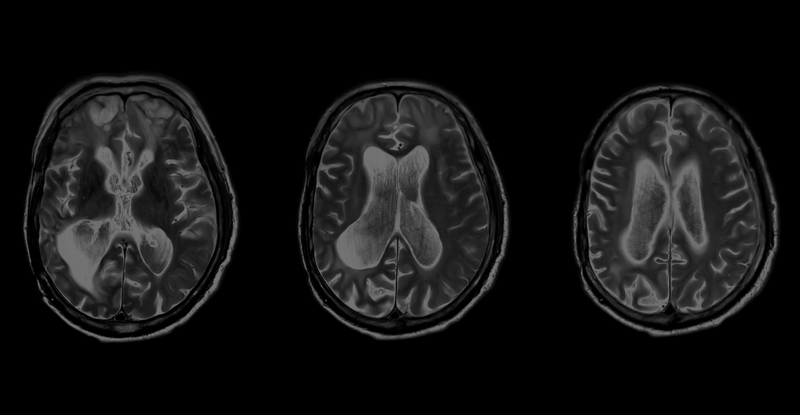
\includegraphics[width=10cm]{images/inputs/brains.png}
		\paragraph{خروجی برنامه}
		یک تصویر به صورت زیر است :\\
		\vspace{0.5cm}\\
		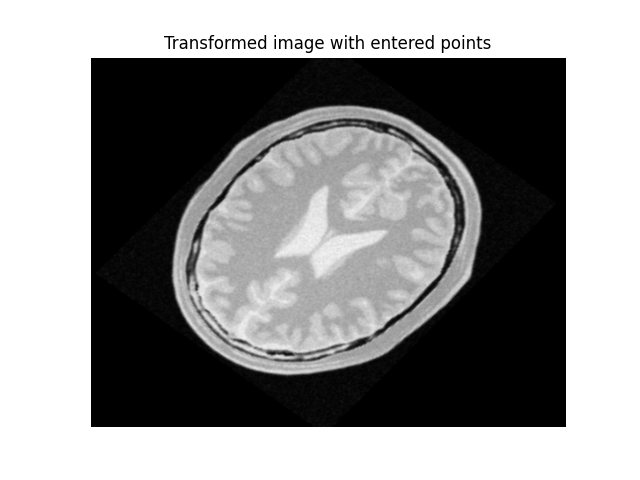
\includegraphics[width=17cm]{images/1.png}
		\newpage
		\section{سوال دوم }
		\paragraph{توضیحات تکمیلی روند کد}
		دو تابع 
		\lr{s1,s2}
		دارای ورودی شدت و خروجی شدت هستند که مطابق با مقاویر خواسته شده، مقادیری را بر میگرداند.
		
		کیفیت تصویر کاهش یافته است اما برای مثال در اینجا ، میتواند به خوبی برخی از اجسام را از محیط اطراف جدا کند و نمایش دهد.
		در تابع دومی نیز، با این کار برخی از شدت هایی که ما را از هدف اصلی عکس دور میکند را حذف کرده ایم.
		
		
		
		\paragraph{ورودی برنامه}
		تصویر زیر ورودی برنامه است \\
		\vspace{0.5cm}\\
		\includegraphics[width=5cm]{images/inputs/kidney.png}
		\paragraph{خروجی برنامه}
			یک تصویر به صورت زیر است:\\
		\vspace{0.5cm}\\
		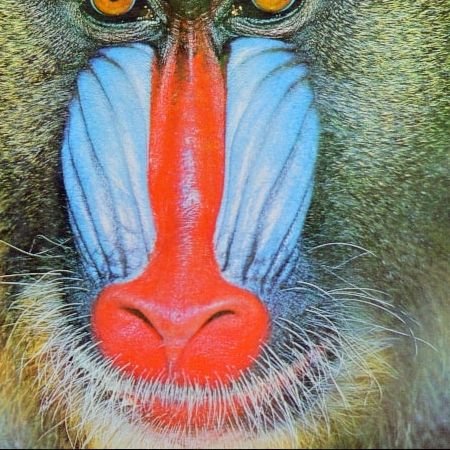
\includegraphics[width=15cm]{images/2.png}
		\newpage
		\section{سوال سوم }
		\paragraph{توضیحات تکمیلی روند کد}
	ابتدا تصاویر ورودی را می گیریم و مطابق فرمول زیر، عملیات 
	\lr{Histogram equalization}
	را اعمال می کنیم :
	
	$p_r(r_k) = \frac{n_k}{MN}$
	
		سپس مطابق فرمول زیر ، این تبدیل را روی تصویر اعمال می کنیم.
		
		
		$s_k = (L-1) \sum_{j=0}^{k} p_r(r_j) $
		
		\paragraph{ورودی برنامه}
		سه تصویر زیر ورودی برنامه است \\
		\vspace{0.5cm}\\
		\includegraphics[width=5cm]{images/inputs/Dark.png}
		\includegraphics[width=5cm]{images/inputs/Bright.png}
		\includegraphics[width=5cm]{images/inputs/Lowcontrast.png}
		\paragraph{خروجی برنامه}
		سه نمودار به صورت زیر است:\\
		\vspace{0.5cm}\\
		\includegraphics[width=10cm]{images/3-1.png}\\
		\includegraphics[width=10cm]{images/3-2.png}\\
		\includegraphics[width=10cm]{images/3-3.png}
		
		\newpage
		\section{سوال چهارم }
		\paragraph{توضیحات تکمیلی روند کد}
		برای فیلتر کردن به صورت دستی مانند الگوریتم ، فیلتر را در تصویرمان ضرب میکنیم. بدین منظور، ابتدا یک پیکسل به اطراف تصویرمان اضافه میکنیم و سپس فیلتر را اعمال می کنیم. 
		برای فیلتر 
		\lr{median}
		نیز دقیقا از الگوریتم اصلی آن استفاده میکنیم به صورتی که در هر پیکسل، در آن 9 پیکسل اطراف ، آن ها را مرتب کرده و مقدا میانی آن را باز میگردانیم .
		در تصویر پویا نیز ، از این تصویر به دست آمده استفاده میکنیم و به ازای مقادیر مختلف اسلایدر ، فیلتر لاپلاسین را به آن اضافه می کنیم. همچنین برای نمایش هیستوگرام در آن نیز هربار تغییر اسلایدر باید هیستوگرام را مجددا رسم نماییم.	
		
		\paragraph{ورودی برنامه}
		تصویر زیر ورودی برنامه است \\
		\vspace{0.5cm}\\
		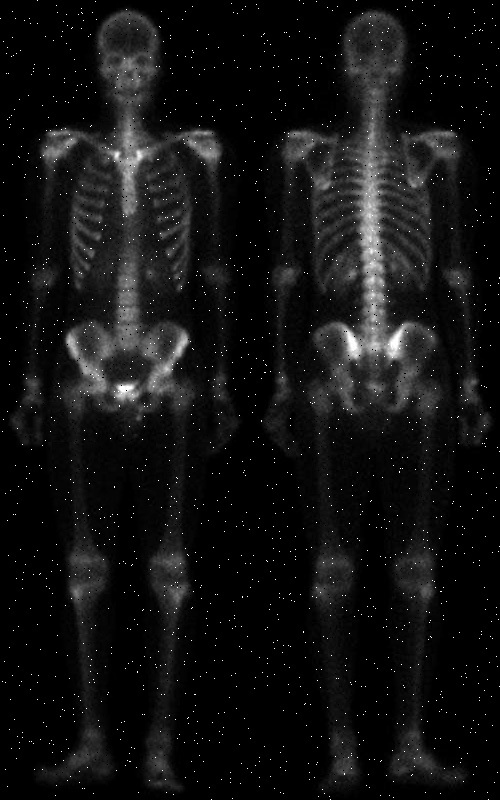
\includegraphics[width=5cm]{images/inputs/bone-scan.png}
		\paragraph{خروجی برنامه} 
		دو تصویر به صورت زیر ، یک تصویر پویا و 
		\lr{True}
		 است:\\
		\vspace{0.5cm}\\
		\includegraphics[width=15cm]{images/4-1.png}\\
		\includegraphics[width=15cm]{images/4-2.png}\\
		\includegraphics[width=15cm]{images/4-3.png}\\
		\includegraphics[width=15cm]{images/4-4.png}\\
		\includegraphics[width=15cm]{images/4-5.png}
		
		
	\newpage
	\raggedleft
	
\end{document}
